% !TeX document-id = {d7bfea81-c3f6-4000-b3a4-ebfa033e41d4}
% !TeX root = ./main.tex
% !TEX program = xelatex
% !BIB program = biber
% !TEX encoding = UTF-8 Unicode
% !TEX options = --shell-escape -synctex=1 -interaction=nonstopmode -file-line-error "%DOC%"
\documentclass{kuee_en}

% if your prefer Times New Roman in Windows, pleas uncomment the below two lines.
% \usepackage{fontspec}
% \setmainfont{Times New Roman}
% and comment these two line
\usepackage[T1]{fontenc}
\usepackage{mathptmx}


% using modern biblatex
\bibliography{sample}

\title{An English \LaTeX{} Template for KUEE}
\etitle{An English \LaTeX{} Template for KUEE}
\eauthor{Denki Jiro} 
\author{{電気 次郎}} % if no kanji name, remove  env.
\supervisor{{電気 太郎 教授}}
\school{{京都大学大学院工学研究科}}
\depart{{電子工学専攻}}
\date{{令和2年2月1日}}

\begin{document}
\maketitle

\begin{abstract}
    \lipsum[1]
\end{abstract}

\tableofcontents

\chapter{Introduction}
This template is designed for the english writer in KUEE.

\lipsum[3-7]

\chapter{Usage}

\section{CJK Languages}

CJKutf8 is used in this paper to generate the cover page and the default font is Meicho font.


\begin{quote}
電気電子工学は現代のあらゆる産業や社会生活の基盤として欠くことのできない科学技術となっています
\end{quote}

\section{Formula for scientists}

Multiple-line aligned example, Maxwell Equations
\begin{align*}
    \div{\vb{D}} &= 0 \\
    \div{\vb{B}} &= 0 \\
    \curl{\vb{E}} &= -\pdv{\vb{B}}{t} \\
    \curl{\vb{H}} &= \pdv{\vb{D}}{t}
\end{align*}

Schr\"{0}edinger Equation
$$
    i\hbar \pdv{\ket{\varphi}}{t} = \mathcal{H} \ket{\varphi}
$$

Chemical equation example
$$
    2\ce{H2}+\ce{O2} = 2\ce{H2O}
$$

\section{Reference and Citation}
Cite this paper
\cite{Yang2007}

\section{Figure and Graph}
A tikz figure shown in Fig. \ref{fig:tikz} and automatically floated to the file end.

\begin{figure}
    \centering
    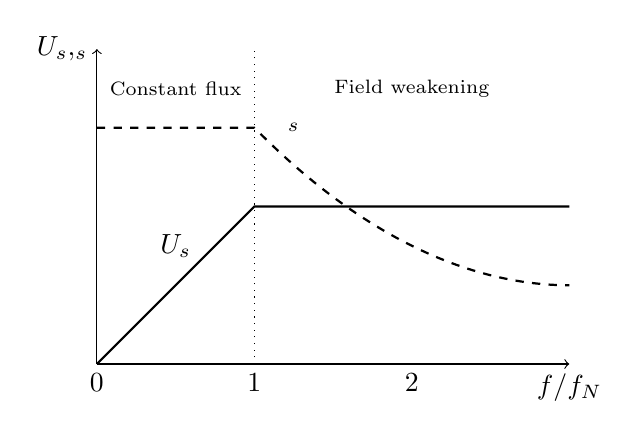
\begin{tikzpicture}
    % horizontal axis
    \draw[->] (0,0) -- (6,0) node[anchor=north] {$f/f_N$};
    % labels
    \draw	(0,0) node[anchor=north] {0}
    		(2,0) node[anchor=north] {1}
    		(4,0) node[anchor=north] {2};
    % ranges
    \draw	(1,3.5) node{{\scriptsize Constant flux}}
    		(4,3.5) node{{\scriptsize Field weakening}};
    % vertical axis
    \draw[->] (0,0) -- (0,4) node[anchor=east] {$U_s,\varPsi_s$};
    % nominal speed
    \draw[dotted] (2,0) -- (2,4);
    % Us
    \draw[thick] (0,0) -- (2,2) -- (6,2);
    \draw (1,1.5) node {$U_s$}; %label
    % Psis
    \draw[thick,dashed] (0,3) -- (2,3) parabola[bend at end] (6,1);
    \draw (2.5,3) node {$\varPsi_s$}; %label
    \end{tikzpicture}
  \caption{A tikz figure example}
  \label{fig:tikz}
\end{figure}


\section{Layout and Parameters}
Default parameters used in this template is shown in Tab.\ref{tab:text}, Tab.\ref{tab:fig}.

\begin{table}
  \caption{Default layout}\label{tab:text}
  \begin{center}
    \begin{tabular}{|l|r|}
      \hline
      \verb+\textwidth+ & 424pt \\ \hline
      \verb+\textheight+ & 604pt \\ \hline
      \verb+\oddsidemargin+ & 0.5cm \\ \hline
      \verb+\evensidemargin+ & 0.5cm \\ \hline
      \verb+\topmargin+ & 0pt \\ \hline
      \verb+\headheight+ &12pt \\ \hline
      \verb+\headsep+ & 25pt \\ \hline
      \verb+\footskip+ & 30pt \\ \hline
    \end{tabular}
  \end{center}
\end{table}

\begin{table}
  \caption{Default parameters for graphs}\label{tab:fig}
  \begin{center}
    \begin{tabular}{|l|r|}
      \hline
      \verb+\textwidth+ & 424pt + 1cm \\ \hline
      \verb+\textheight+ & 604pt + 67pt \\ \hline
      \verb+\oddsidemargin+ & 0pt \\ \hline
      \verb+\evensidemargin+ & 0pt \\ \hline
      \verb+\topmargin+ & 0pt \\ \hline
      \verb+\headheight+ & 0pt \\ \hline
      \verb+\headsep+ & 0pt \\ \hline
      \verb+\footskip+ & 0pt \\ \hline
    \end{tabular}
  \end{center}
\end{table}


\chapter{Lorem}
\lipsum[2-5]

\chapter{Ipsum}
\lipsum[4-8]

\begin{acknowledgements}
\lipsum[2]
\end{acknowledgements}

\printbibliography[title=References,heading=bibintoc]

\clearpage % ensure all floats are processed
\processdelayedfloats
\clearpage

\begin{appendices}
\chapter{Versions}
\begin{description}
  \item[2019] 1st version by Zhenghao Yin, Takeuchi lab.
\end{description}
\end{appendices}


\end{document}

